\documentclass{article}

%Aus dem LaTex Template der Universit�t Stuttgart
%------------------------------------------------
\usepackage[utf8]{inputenc}
\usepackage[T1]{fontenc}
\usepackage[sfdefault]{ClearSans} %% option 'sfdefault' activates Clear Sans as the default text font
\usepackage{cmap}
\usepackage[ngerman]{babel}
\usepackage{graphicx}
\usepackage[pdftex,hyperref,dvipsnames]{xcolor}
\usepackage{listings}
\usepackage[a4paper,lmargin={2cm},rmargin={2cm},tmargin={3.5cm},bmargin = {2.5cm},headheight = {4cm}]{geometry}
\usepackage{amsmath,amssymb,amstext,amsthm}
\usepackage[lined,algonl,boxed]{algorithm2e}
\usepackage{tikz}
\usepackage{hyperref}
\usepackage{url}
\usepackage[inline]{enumitem} % Erm�glicht �ndern der enum Item Zahlen
\usepackage[headsepline]{scrpage2} 
\usepackage{algorithmic} % F�r Pseudocode
\usepackage{ marvosym } % f�r Pfeil(e)
\usepackage{booktabs} % F�r die sch�neren Booktabs-Tabellen
\usepackage{tikz}
\usepackage{pdfpages}
\usepackage{blindtext}
\usepackage{scrextend}
\usepackage{pdfpages}
\usepackage{natbib} % Yannis hat das importiert; TODO: nachfragen, zu was das gut ist
\pagestyle{scrheadings} 
\usetikzlibrary{automata,positioning}
\usepackage{lscape}

\begin{document}
	 % Counter für das Blatt und die Aufgabennummer.
% Ersetze die Nummer des Übungsblattes und die Nummer der Aufgabe
% den Anforderungen entsprechend.
% Beachte:
% \setcounter{countername}{number}: Legt den Wert des Counters fest
% \stepcounter{countername}: Erhöht den Wert des Counters um 1.
\newcounter{sheetnr}
\setcounter{sheetnr}{1} % Nummer des Übungsblattes
\newcounter{exnum}
\setcounter{exnum}{1} % Nummer der Aufgabe

% Befehl für die Aufgabentitel
\newcommand{\exercise}[1]{\section*{Aufgabe \theexnum\stepcounter{exnum} #1}} % Befehl für Aufgabentitel

% Formatierung der Kopfzeile
% \ohead: Setzt rechten Teil der Kopfzeile mit
% Namen und Matrikelnummern aller Bearbeiter
\ohead{Yannis Blosch (3256958)\\
Lukas Heiland (3269754)}
% \chead{} kann mittleren Kopfzeilen Teil sezten
% \ihead: Setzt linken Teil der Kopfzeile mit
% Modulnamen, Semester und Übungsblattnummer
\ihead{Modellierung\\
Sommersemester 2018\\
Blatt \thesheetnr}
	 
	 \section*{Aufgabe 9.1}
	 ... befindet sich auf der nächsten Seite. Warum? Weil LaTeX das so will :(
	 	\begin{landscape}
	 		\begin{figure}[h!]
	 			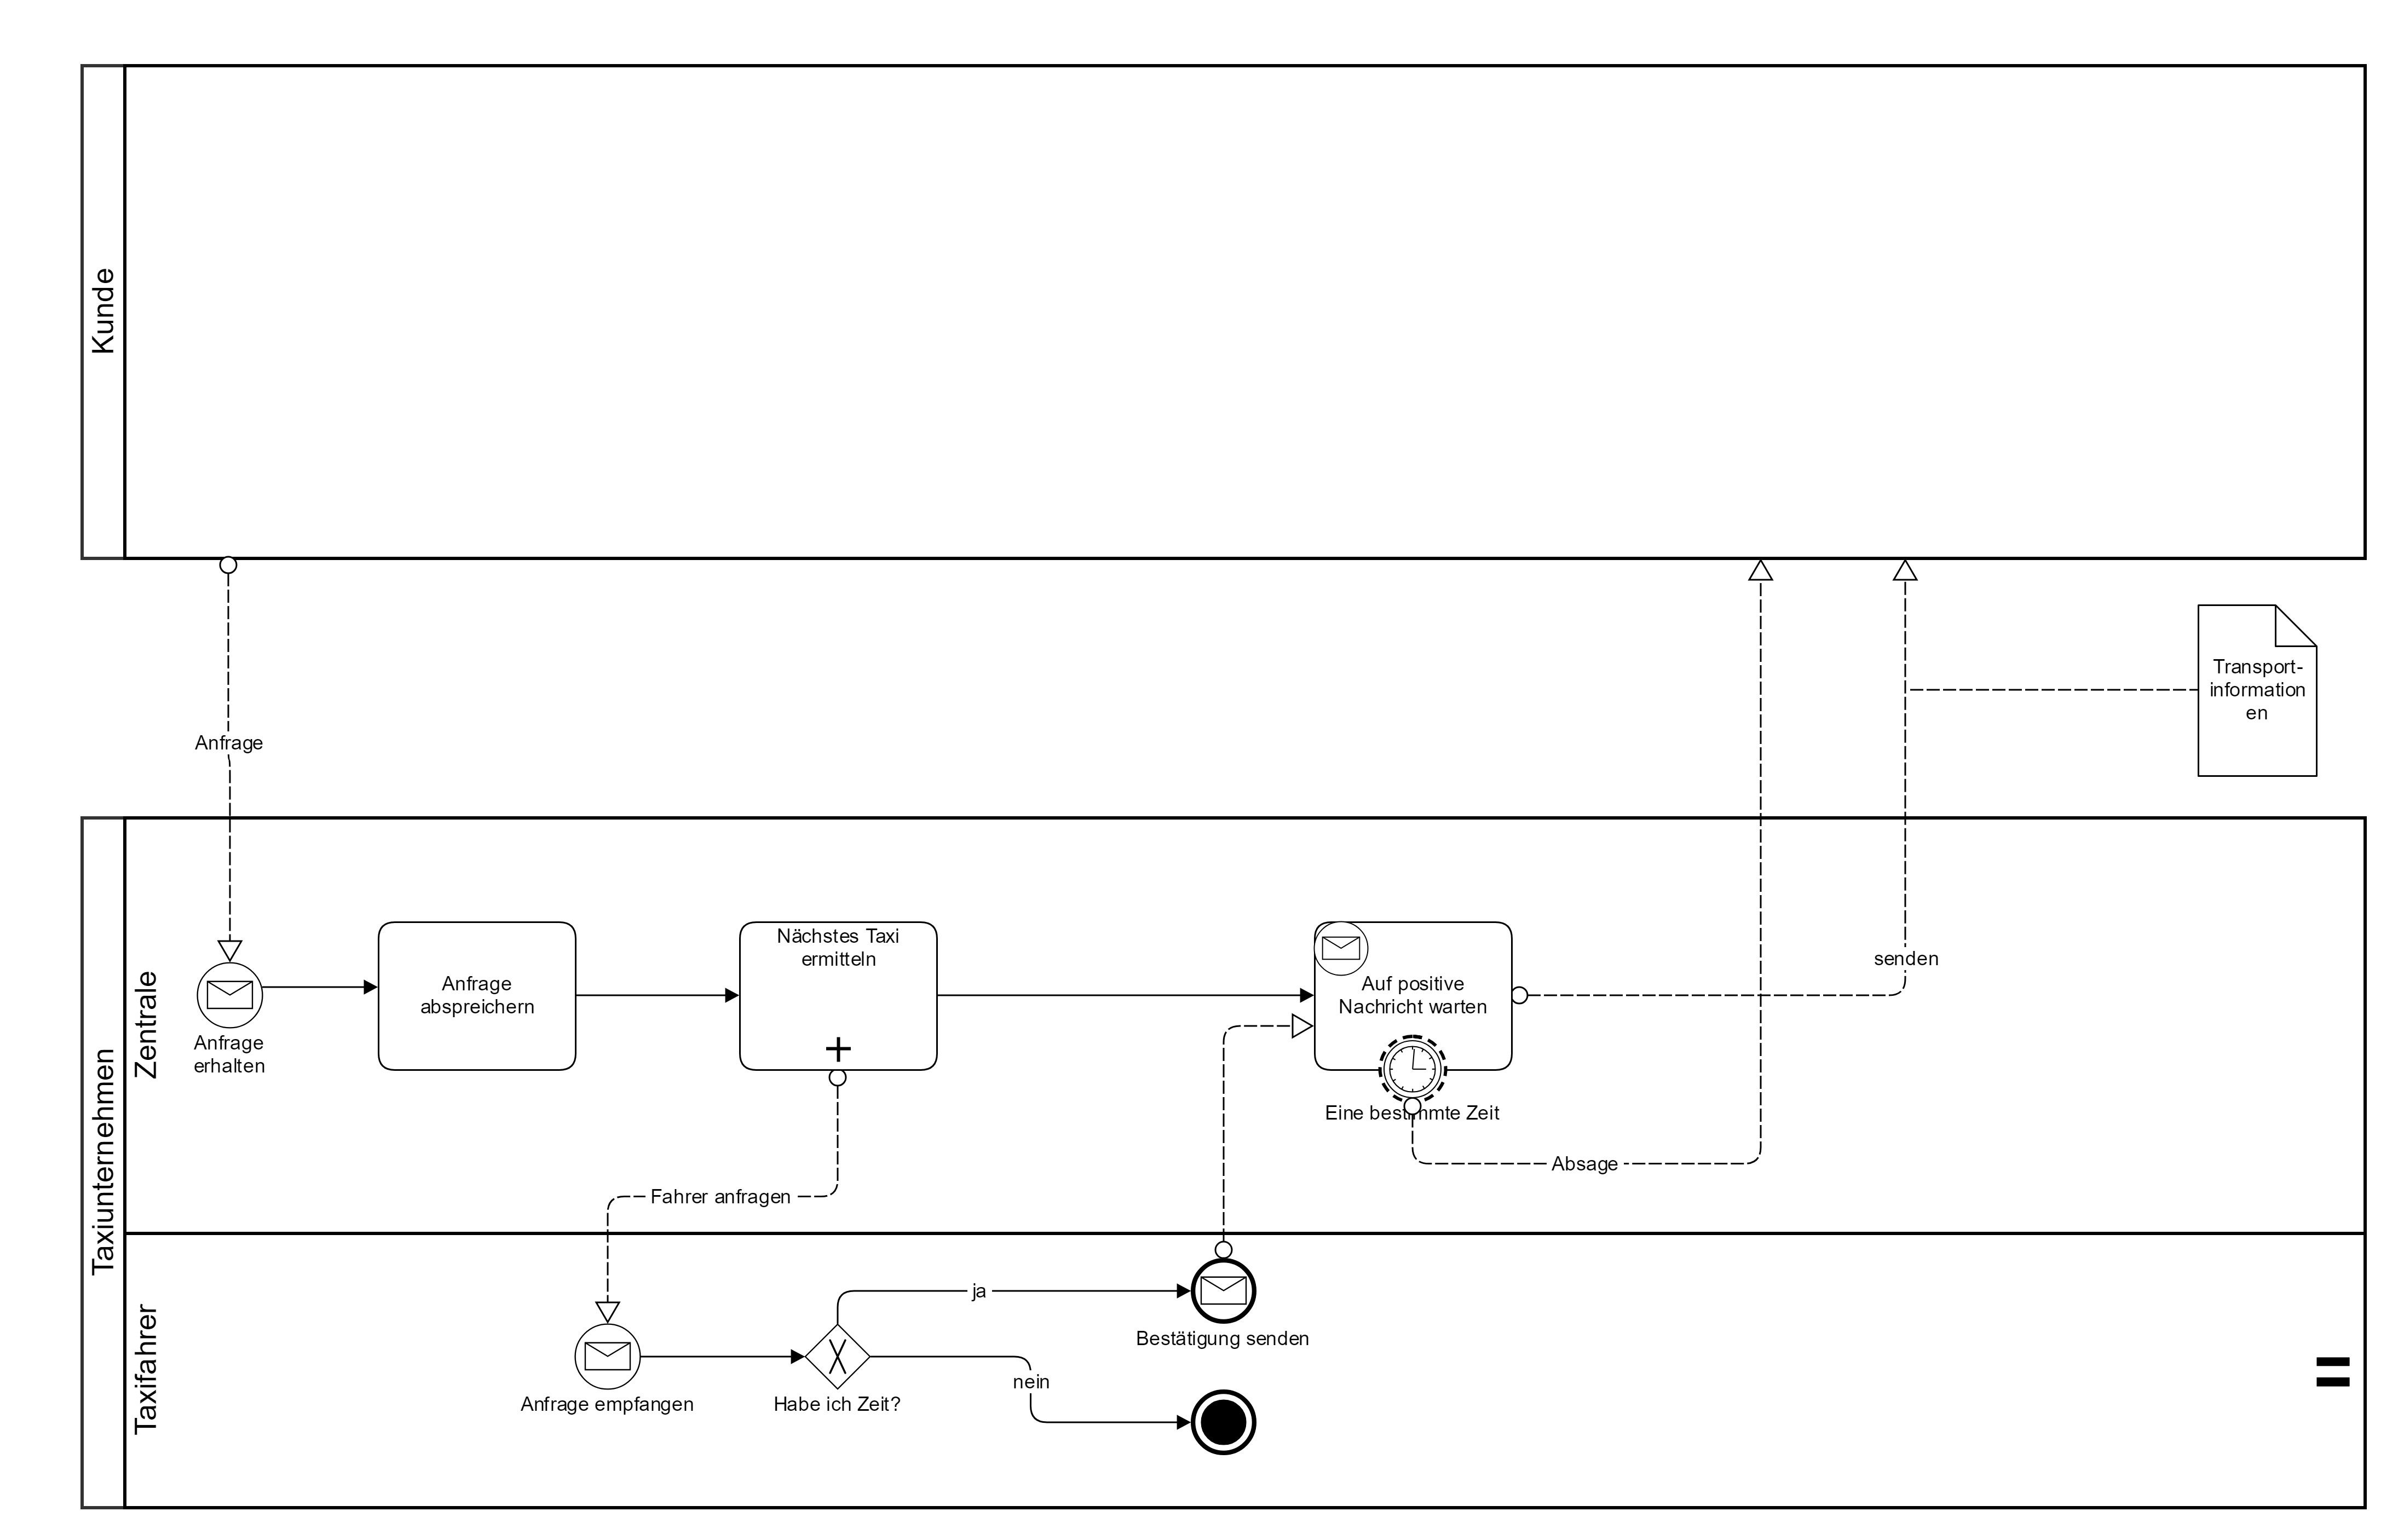
\includegraphics[scale=0.14]{aufgabe_9_1.jpg}
	 		\end{figure}
	 	\end{landscape}
	
	
	\section*{Aufgabe 9.2}
	%%% TODO %%%
	\pagebreak
	
	
	\section*{Aufgabe 9.3}
		\subsection*{a)}
			\begin{figure}[h!]
				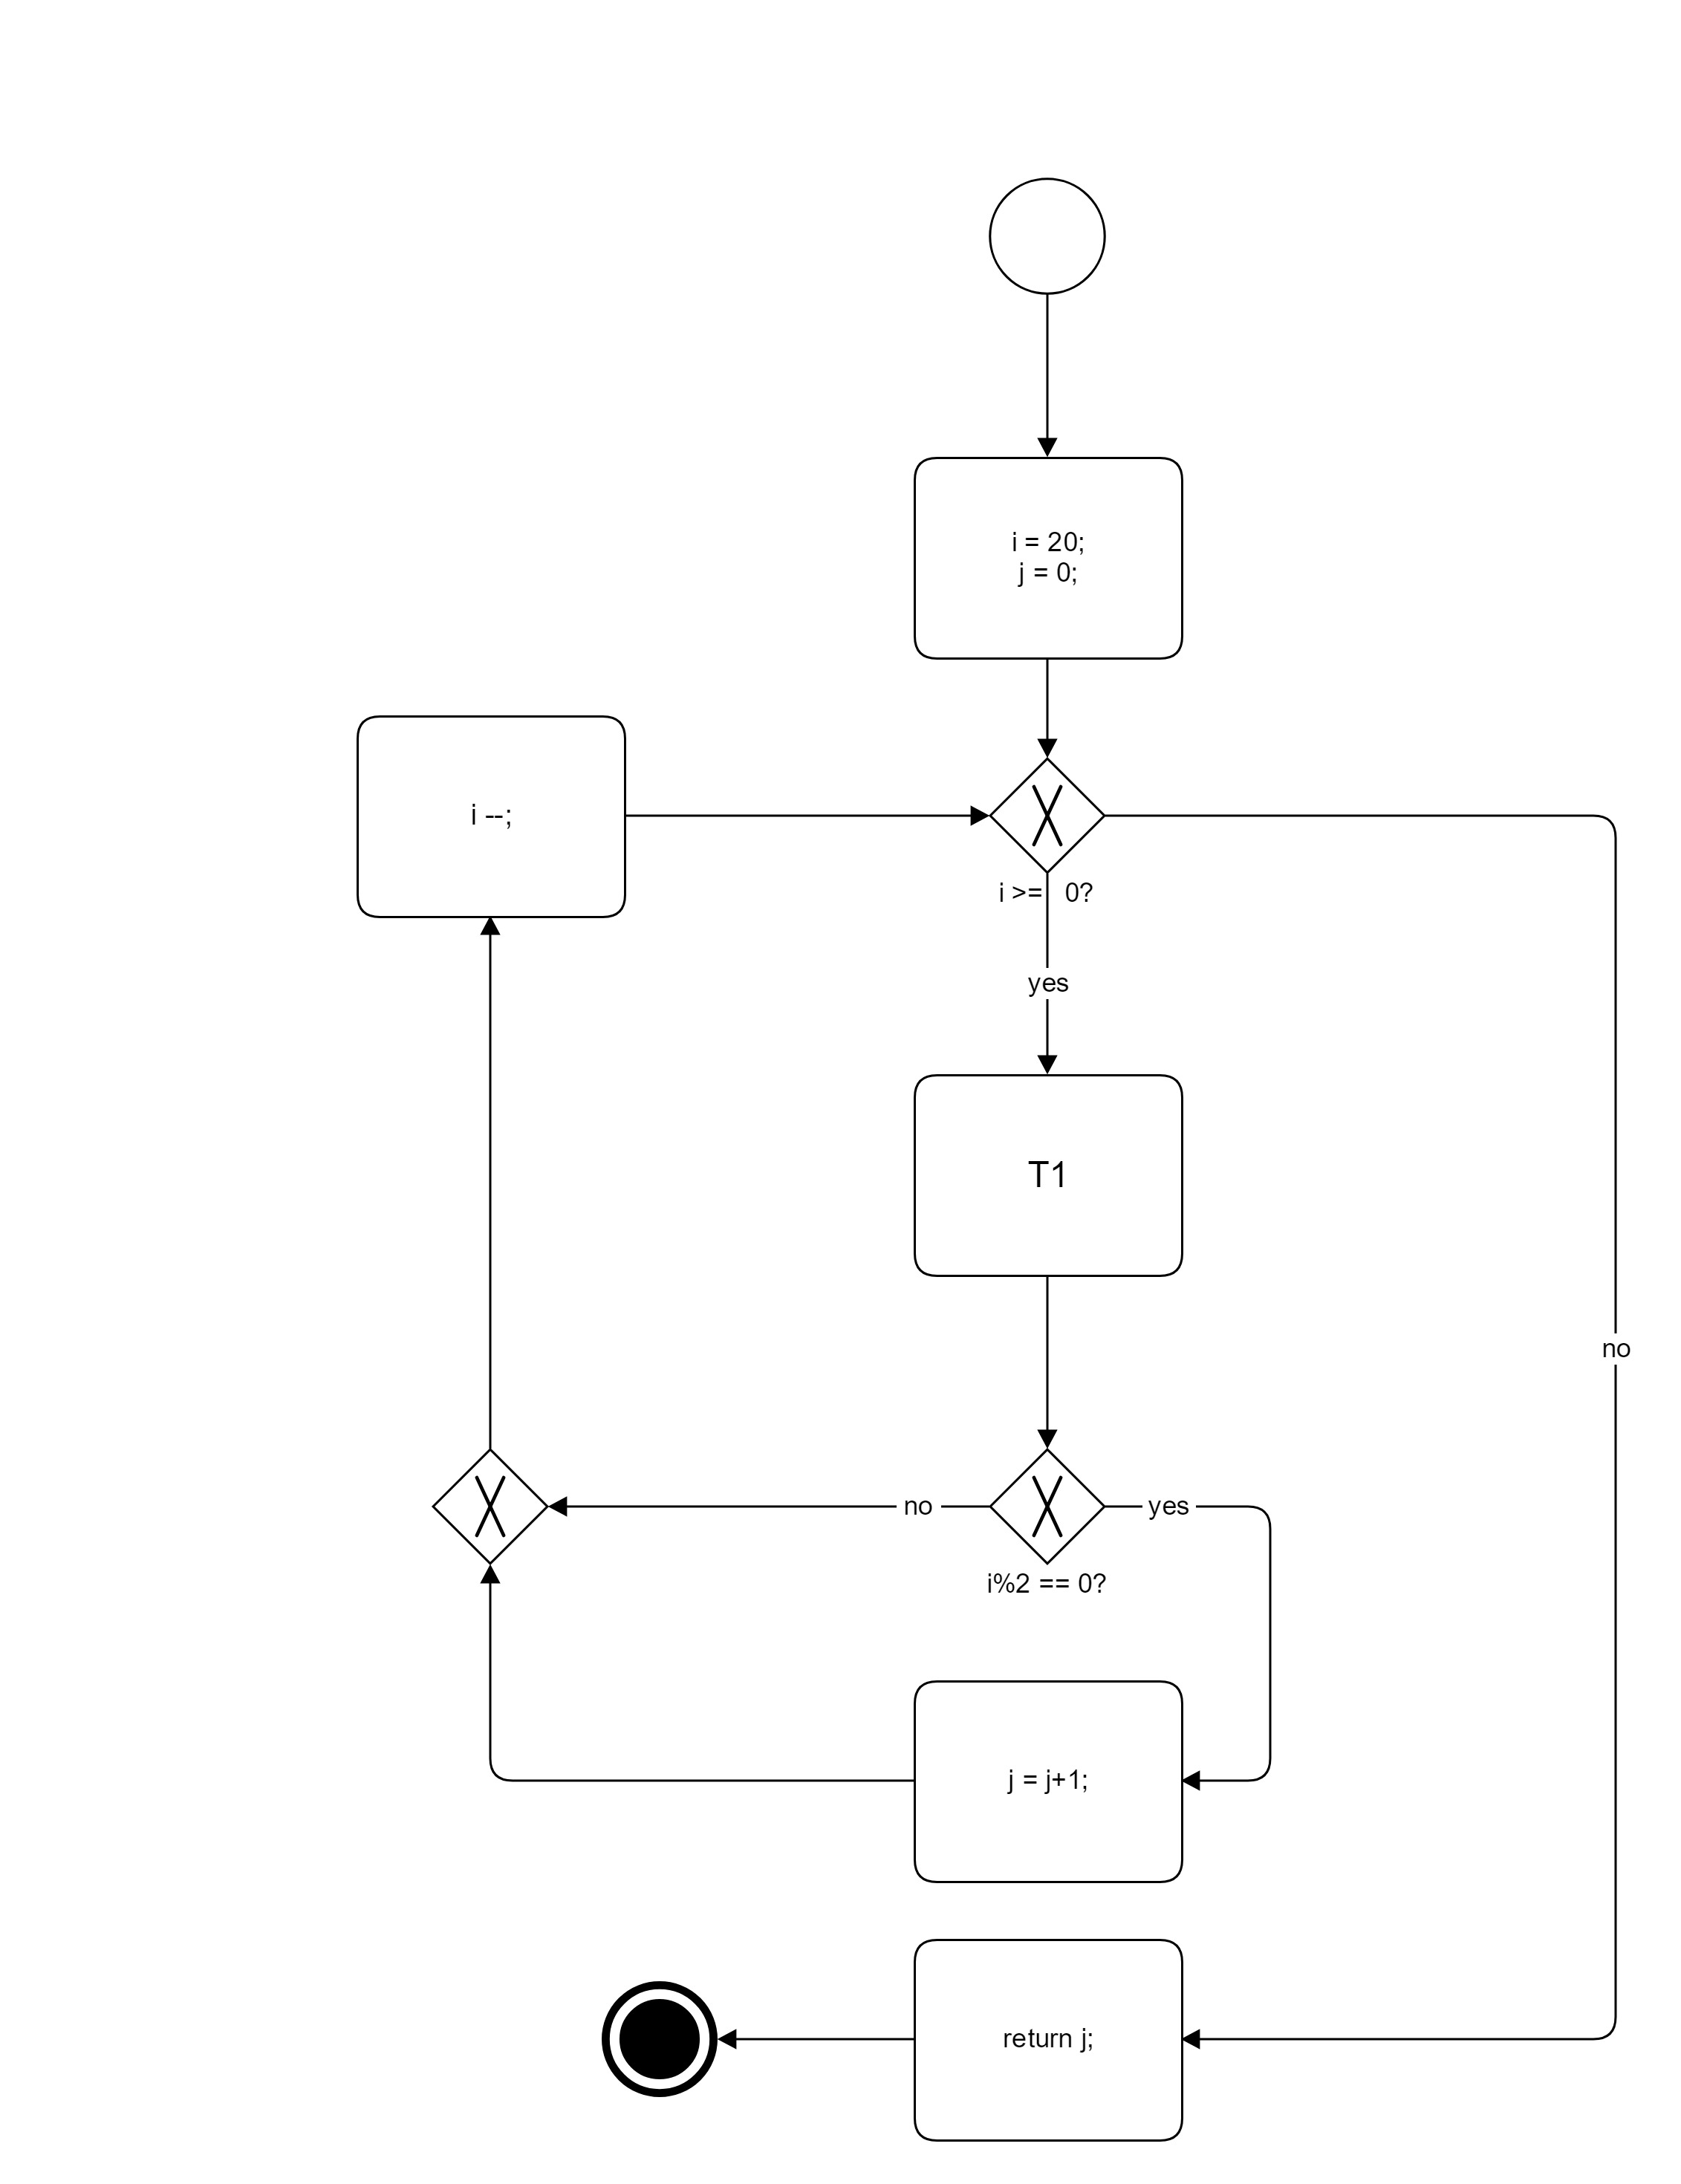
\includegraphics[scale=0.2]{aufgabe_9_3_a.jpg}
			\end{figure}
		
	\pagebreak
	
		\subsection*{b)}
			\begin{figure}[h!]
				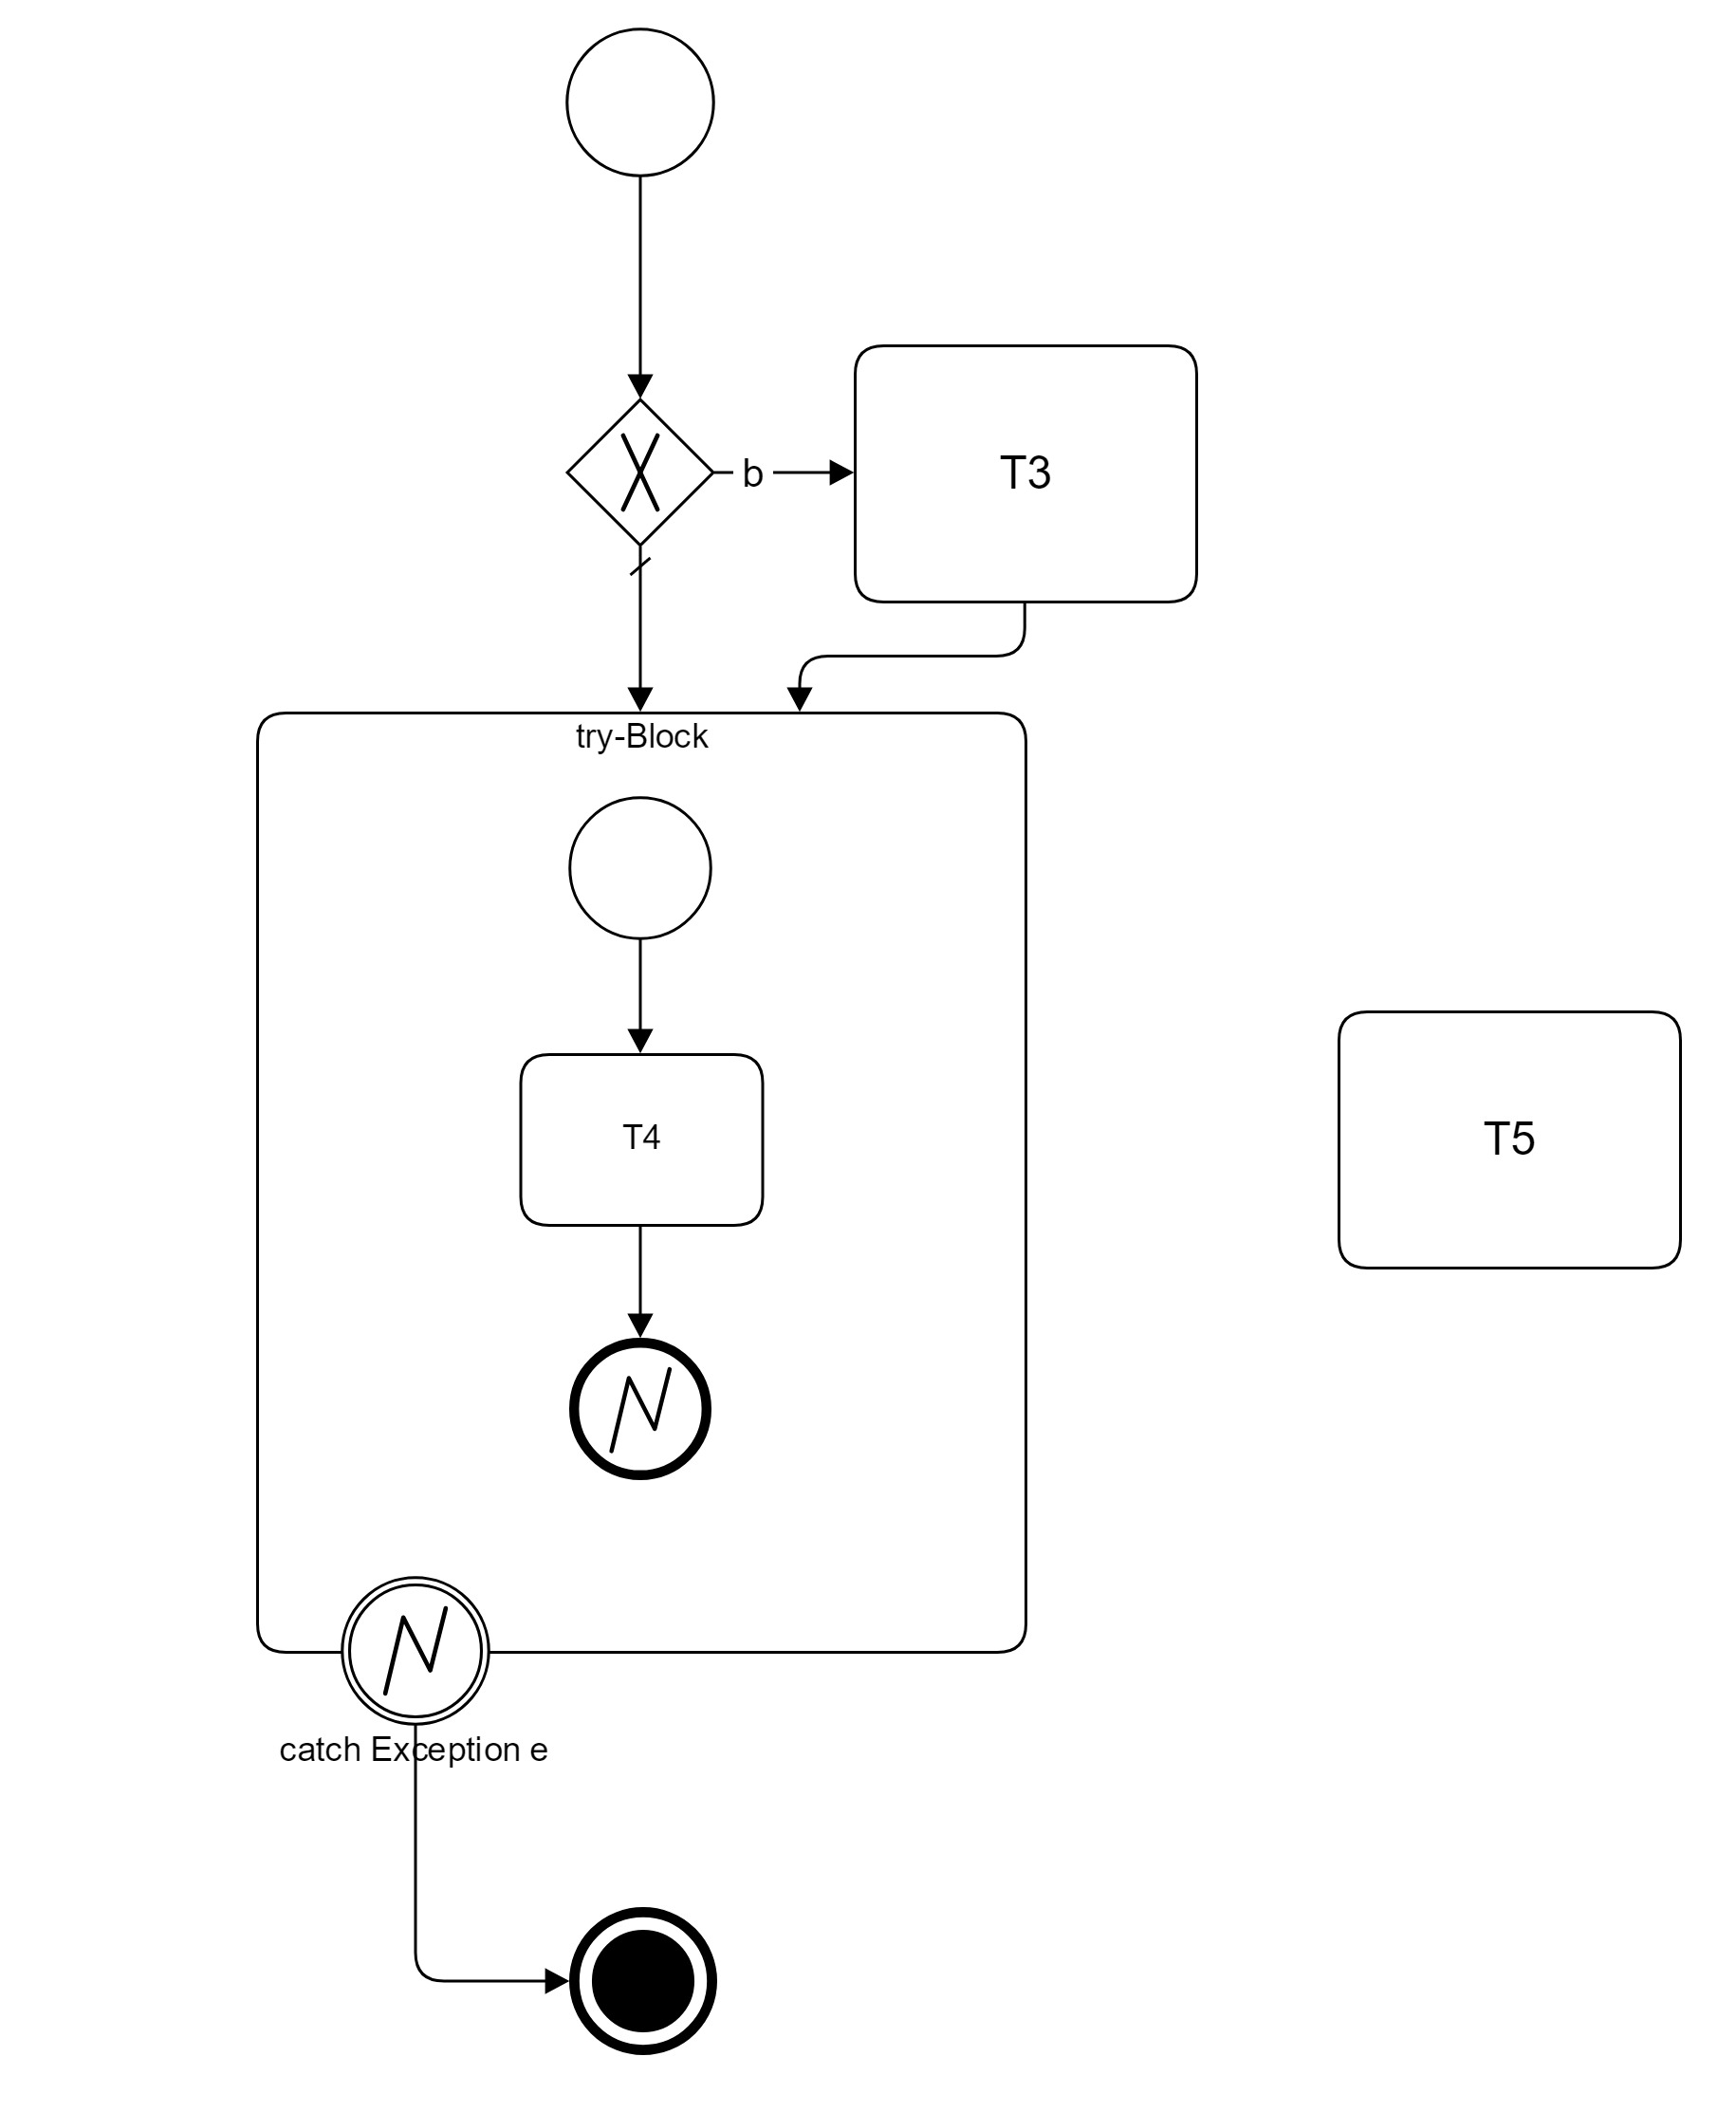
\includegraphics[scale=0.25]{aufgabe_9_3_b.jpg}
			\end{figure}
		
	\pagebreak
		
	\section*{Aufgabe 9.4}
		\begin{table}[h!]
			\begin{tabular}{l|l|l|l}
				& message rcv & message send & message catch \\ \hline
				\textbf{Platzhalter 1} &  J           &  J            &  N             \\ \hline
				\textbf{Platzhalter 2} &  N           &  N            &  J             \\ \hline
				\textbf{Platzhalter 3} &  J           &  J            &  N             \\ \hline
				\textbf{Platzhalter 4} &  N           &  J            &  N            
			\end{tabular}
		\end{table}
			
\end{document}